\documentclass{article}

\usepackage{amsmath, amsfonts, amssymb, amsthm}
\usepackage[utf8]{inputenc}
\usepackage[spanish, mexico]{babel}
\selectlanguage{spanish}
\usepackage[margin=0.5in]{geometry}
\usepackage{graphicx}

\title{Taller 2: Teoría de números}
\author{Miguel A. Gomez B.}

\begin{document}
	
	\maketitle
	
\paragraph{Ejercicio 1} Verifique, usando el principio del buen orden, que el conjunto $S = \{ 2x + 3y: x, n \in \mathbb{Z} \}$ tiene un elemento positivo mínimo y calcular este elemento.

\begin{proof}
Nos interesa demostrar la existencia de un número positivo por lo tanto construímos un nuevo conjunto que contiene los enteros positivos del conjunto $S$ (un subconjunto) y que llamaremos $S^+$, así:

\begin{equation}\label{eq:1}
S^+ = \{2x + 3y : x,y \in \mathbb{Z} \land 2x + 3y \ge 0\}
\end{equation}

Ahora debemos demostrar que $S$ es un conjunto no vacío para que se cumpla el principio del buen orden. Y en efecto es así, siempre y cuando $x\geq0$ e $y\geq0$, su suma también lo será, por la definición de suma de los números enteros positivos.

\paragraph{}
Hay dos casos más

\subparagraph{Caso I: $x<0$.} Si $2x < 0$, entonces para que se mantenga la construcción de $S^+$ se debe cumplir que $2x < 3y \geq |2x|$. Por ejemplo:
\begin{center}
	Si $x=-3$ e $y=2$, entonces
	\[
	2(-3) + 3(2) = -6 + 6 = 0
	\]
	Y siempre y cuando $3y = |2x| + n$ con $n \in \mathbb{N}$.
\end{center}

\subparagraph{Caso II: $y<0$.} Si $3y < 0$, entonces para que se mantenga la construcción de $S^+$ se debe cumplir que $3y < 2x \geq |3y|$. Por ejemplo (análogo al caso anterior):

\begin{center}
	Si $x=3$ e $y=-2$, entonces
	\[
	2(3) + 3(-2) = 6 - 6 = 0
	\]
	Y siempre y cuando $2x = |3y| + n$ con $n \in \mathbb{N}$.
\end{center}

Lo que demuestra que $S^+$ es no vacío. Luego por el principio del buen orden $S^+$ posee un elemento mínimo, lo cual implica que la parte positiva de $S$ tiene un mínimo y como vimos en los ejemplos anteriores, es el número $0$.
\end{proof}

\paragraph{Ejercicio 2} Prueba usando el principio de inducción, las fórmulas para $S_n$, $t_n$ y $T_n$.

\begin{equation} \label{eq:2}
	S_n = 1 + 3 +5 + \dots + 2n - 1 = n^2 
\end{equation}

\begin{equation}\label{eq:3}
	t_n = 1 + 2 + \dots + n - 1  + n = \frac{n(n+1)}{2}
\end{equation}

\begin{equation}\label{eq:4}
	T_n = t_1 + t_2 + \dots + t_n = \frac{n(n+1)(n+2)}{6}
\end{equation}

\begin{proof}(Por inducción para (\ref{eq:2})). La igualdad se cumple para $n=1$ pues $1 = 1^2 = 1$.
	
\subparagraph{Hipótesis de inducción.} Suponemos que la proposición es verdadera para $n=k$, es decir:

	\begin{equation}\label{eq:2_1}
		1 + 3 + 5 + \dots + 2k-1 = k^2
	\end{equation}

Ahora suponemos el siguiente $n = k + 1$ y por ende tenemos:

\[
	1 + 3 + 5 + \dots + 2k - 1 + 2(k+1) - 1 = (k + 1)^2\\
\]	

sin embargo por la hipótesis de inducción (\ref{eq:2_1}) tenemos ahora:

\[
	k^2 + 2(k+1) - 1 = (k + 1)^2\\
\]

Manipulando algebraicamente la expresión $k^2 + 2(k+1) - 1$ deberíamos obtener $(k + 1)^2$:

\begin{align*}
	k^2 + 2(k+1) - 1 &= k^2 + 2k + 2 - 1 \\
	&= k^2 + 2k + 1\\
	&= (k + 1)^2
\end{align*}

Por lo tanto hemos demostrado que si la proposición es correcta para $n = k$, es correcta para $n=k+1$. Entonces, por el principio de inducción, la fórmula es válida para todo $n \in \mathbb{N}$.

\end{proof}

\begin{proof}(Por inducción para (\ref{eq:3})). La igualdad se cumple para $n=1$ pues $1 = \frac{1(1+1)}{2} = \frac{2}{2} = 1$.
	
\subparagraph{Hipótesis de inducción.} Suponemos que la proposición es verdadera para $n=k$, es decir:

	\begin{equation}\label{eq:3_1}
		1 + 2 + \dots + k -1 + k = \frac{k(k+1)}{2}
	\end{equation}

Ahora suponemos el siguiente $n = k + 1$ y por ende tenemos:

\[
	1 + 2 + \dots + k - 1 + k + (k + 1) = \frac{(k+1)[(k+1)+1]}{2}
\]	

sin embargo por la hipótesis de inducción (\ref{eq:3_1}) tenemos ahora:

\[
	\frac{k(k+1)}{2} + (k + 1) = \frac{(k+1)[(k+1)+1]}{2}
\]

Manipulando algebraicamente la expresión $\frac{k(k+1)}{2} + (k + 1)$ deberíamos obtener $\frac{(k+1)[(k+1)+1]}{2}$:

\begin{align*}
	\frac{k(k+1)}{2} + (k + 1) &= (k+1)\left(\frac{k}{2} + 1\right)\\
	&= (k+1)\left(\frac{k}{2} + \frac{2}{2}\right)\\
	&= (k+1)\left(\frac{k + 2}{2}\right)\\
	&= (k+1)\left(\frac{k + 1 + 1}{2}\right)\\
	&= \frac{(k+1)[(k + 1) + 1]}{2}
\end{align*}

Por lo tanto hemos demostrado que si la proposición es correcta para $n = k$, es correcta para $n=k+1$. Entonces, por el principio de inducción, la fórmula es válida para todo $n \in \mathbb{N}$.
\end{proof}

\begin{proof}(Por inducción para (\ref{eq:4})). La igualdad se cumple para $n=1$ pues $1 = \frac{1(1+1)(1+2)}{6} = \frac{(2)(3)}{6} = \frac{6}{6} = 1$.
	
\subparagraph{Hipótesis de inducción.} Suponemos que la proposición es verdadera para $n=k$, es decir:

	\begin{equation}\label{eq:4_1}
		1 + 3 + \dots + \frac{k(k+1)}{2} = \frac{k(k+1)(k+2)}{6}
	\end{equation}

Ahora suponemos el siguiente $n = k + 1$ y por ende tenemos:

\begin{align*}
    1 + 3 + \dots + \frac{k(k+1))}{2} + \frac{(k+1)[(k+1) + 1]}{2} &= \frac{(k+1)[(k+1) + 1][(k+1)+2]}{6}\\
    1 + 3 + \dots + \frac{k(k+1))}{2} + \frac{(k+1)(k+2)}{2} &= \frac{(k+1)(k+2)(k+3)}{6}
\end{align*}

sin embargo por la hipótesis de inducción (\ref{eq:4_1}) tenemos ahora:

\[
	\frac{k(k+1)(k+2)}{6} + \frac{(k+1)(k+2)}{2} = \frac{(k+1)[(k+1)+1]}{6}
\]

Manipulando algebraicamente la expresión $\frac{k(k+1)(k+2)}{6} + \frac{(k+1)(k+2)}{2}$ deberíamos obtener $\frac{(k+1)(k+2)(k+3)}{6}$:

\begin{align*}
	\frac{k(k+1)(k+2)}{6} + \frac{(k+1)(k+2)}{2} &= \frac{k(k+1)(k+2)}{6} + \frac{3(k+1)(k+2)}{6}\\ &= \frac{k(k+1)(k+2) + 3(k+1)(k+2)}{6}\\
	&= \frac{(k+1)(k+2)(k+3)}{6}
\end{align*}

Por lo tanto hemos demostrado que si la proposición es correcta para $n = k$, es correcta para $n=k+1$. Entonces, por el principio de inducción, la fórmula es válida para todo $n \in \mathbb{N}$.
\end{proof}

\paragraph{Ejercicio 3} Muestre que $8t_n + 1 = S_{2n+1}$.

\begin{proof}(Directa) repesentamos la igualdad $8t_n + 1 = S_{2n+1}$ con sus formulas equivalentes:

\begin{align} \label{eq:5_1}
    8t_n + 1 = \frac{8n(n+1)}{2} + 1
\end{align}

\begin{align}\label{eq:5_2}
    S_{2n+1} = (2n+1)^2
\end{align}

Reemplazando (\ref{eq:5_1}) y (\ref{eq:5_2}) en la igualdad inicial, obtenemos la nueva igualdad:

\begin{equation}\label{eq:5_3}
    \frac{8n(n+1)}{2} + 1 = (2n+1)^2
\end{equation}

Luego manipulando algebraicamente un lado de la igualdad de (\ref{eq:5_3}) deberíamos obtener la otra, elegimos $\frac{8n(n+1)}{2} + 1$, verificando obtenemos:

\begin{align*}
    \frac{8n(n+1)}{2} + 1 &= 4n(n+1) + 1\\
    &= 4n^2 + 4n +1\\
    &= (2n + 1)^2
\end{align*}

Por lo tanto, queda demostrado que las expresiones (\ref{eq:5_1}) y (\ref{eq:5_2}) son equivalentes.
\end{proof}

\paragraph{Ejercicio 3} Escriba un resúmen corto acerca de los números poligonales descritos en la sección 1.4. pero utilice cualquier otro soporte bibliográfico que considere.

\paragraph{} Un número poligonal es un tipo de número figurado, estos tipos de números (los figurados) son números que representan puntos equidistantes y que forman arreglos geométricos regulares. Si estos puntos tienen la forma de un polígono regular (triangulo, curadrado, hexágono, etc) se le conoce como número poligonal, pero también los números figurados pueden asemejarse a otras construcciones geométricas como sólidos.

\begin{center}
    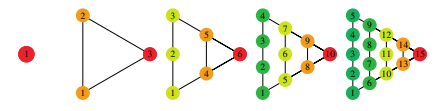
\includegraphics[scale=0.8]{example}
\end{center}

en este caso representa un triángulo y este número se expresa como

$$t_n = 1 + 2 + 3 + \dots + n-1 + n$$

y de manera más general cómo

$$t_n = \frac{n(n+1)}{2}$$

Por ejemplo, el $10$ es un número triangular porque

$$10 = \frac{4(5)}{2} = 10$$

y que también se evidencia en la gráfica. Por esta misma razón 2 no es un número triangular y que también podemos evidenciaren su representación algebráica.

También hay numeros cuadrados

\begin{center}
    
\includegraphics[scale=0.8]{squared}
\end{center}

y podemos ver que tienen una relación con los números triangulares que ya demostramos en el ejercicio anterior

\begin{equation*}
	S_n = 1 + 3 +5 + \dots + 2n - 1 = n^2 
\end{equation*}

e igualmente los números tetraédricos en donde la relación que demostramos, es mucho más estrecha con los números triangulares y que podemos ver en su construcción geométrica y su representación algebráica:

\begin{equation*}
	T_n = t_1 + t_2 + \dots + t_n = \frac{n(n+1)(n+2)}{6}
\end{equation*}

\begin{center}
    
\includegraphics[scale=0.8]{tetraedricos}
\end{center}

Sin embargo los números tetraédricos no son números poligonales dado que existen en un espacio tridimensional, pero sí son números figurados.

\nocite{*}

\bibliography{bibliography}
\bibliographystyle{ieeetr}

\end{document}
